% !TeX document-id = {d8a08665-68b2-4c28-8b7c-81fa3895c963}
% !TEX TS-program = pdflatexmk
\documentclass[10pt,a4paper]{article}
\usepackage[english]{babel}
\usepackage[latin1]{inputenc}
\usepackage{lipsum}
\usepackage{authblk}
\usepackage{amsmath}
\usepackage{amsfonts}
\usepackage{amssymb}
\usepackage{polski}
\usepackage{graphicx}
\usepackage{cite}
\usepackage{listings}
\usepackage{float}
\selectlanguage{english}
\begin{document}
	
	\begin{figure}[H]
		\centering
		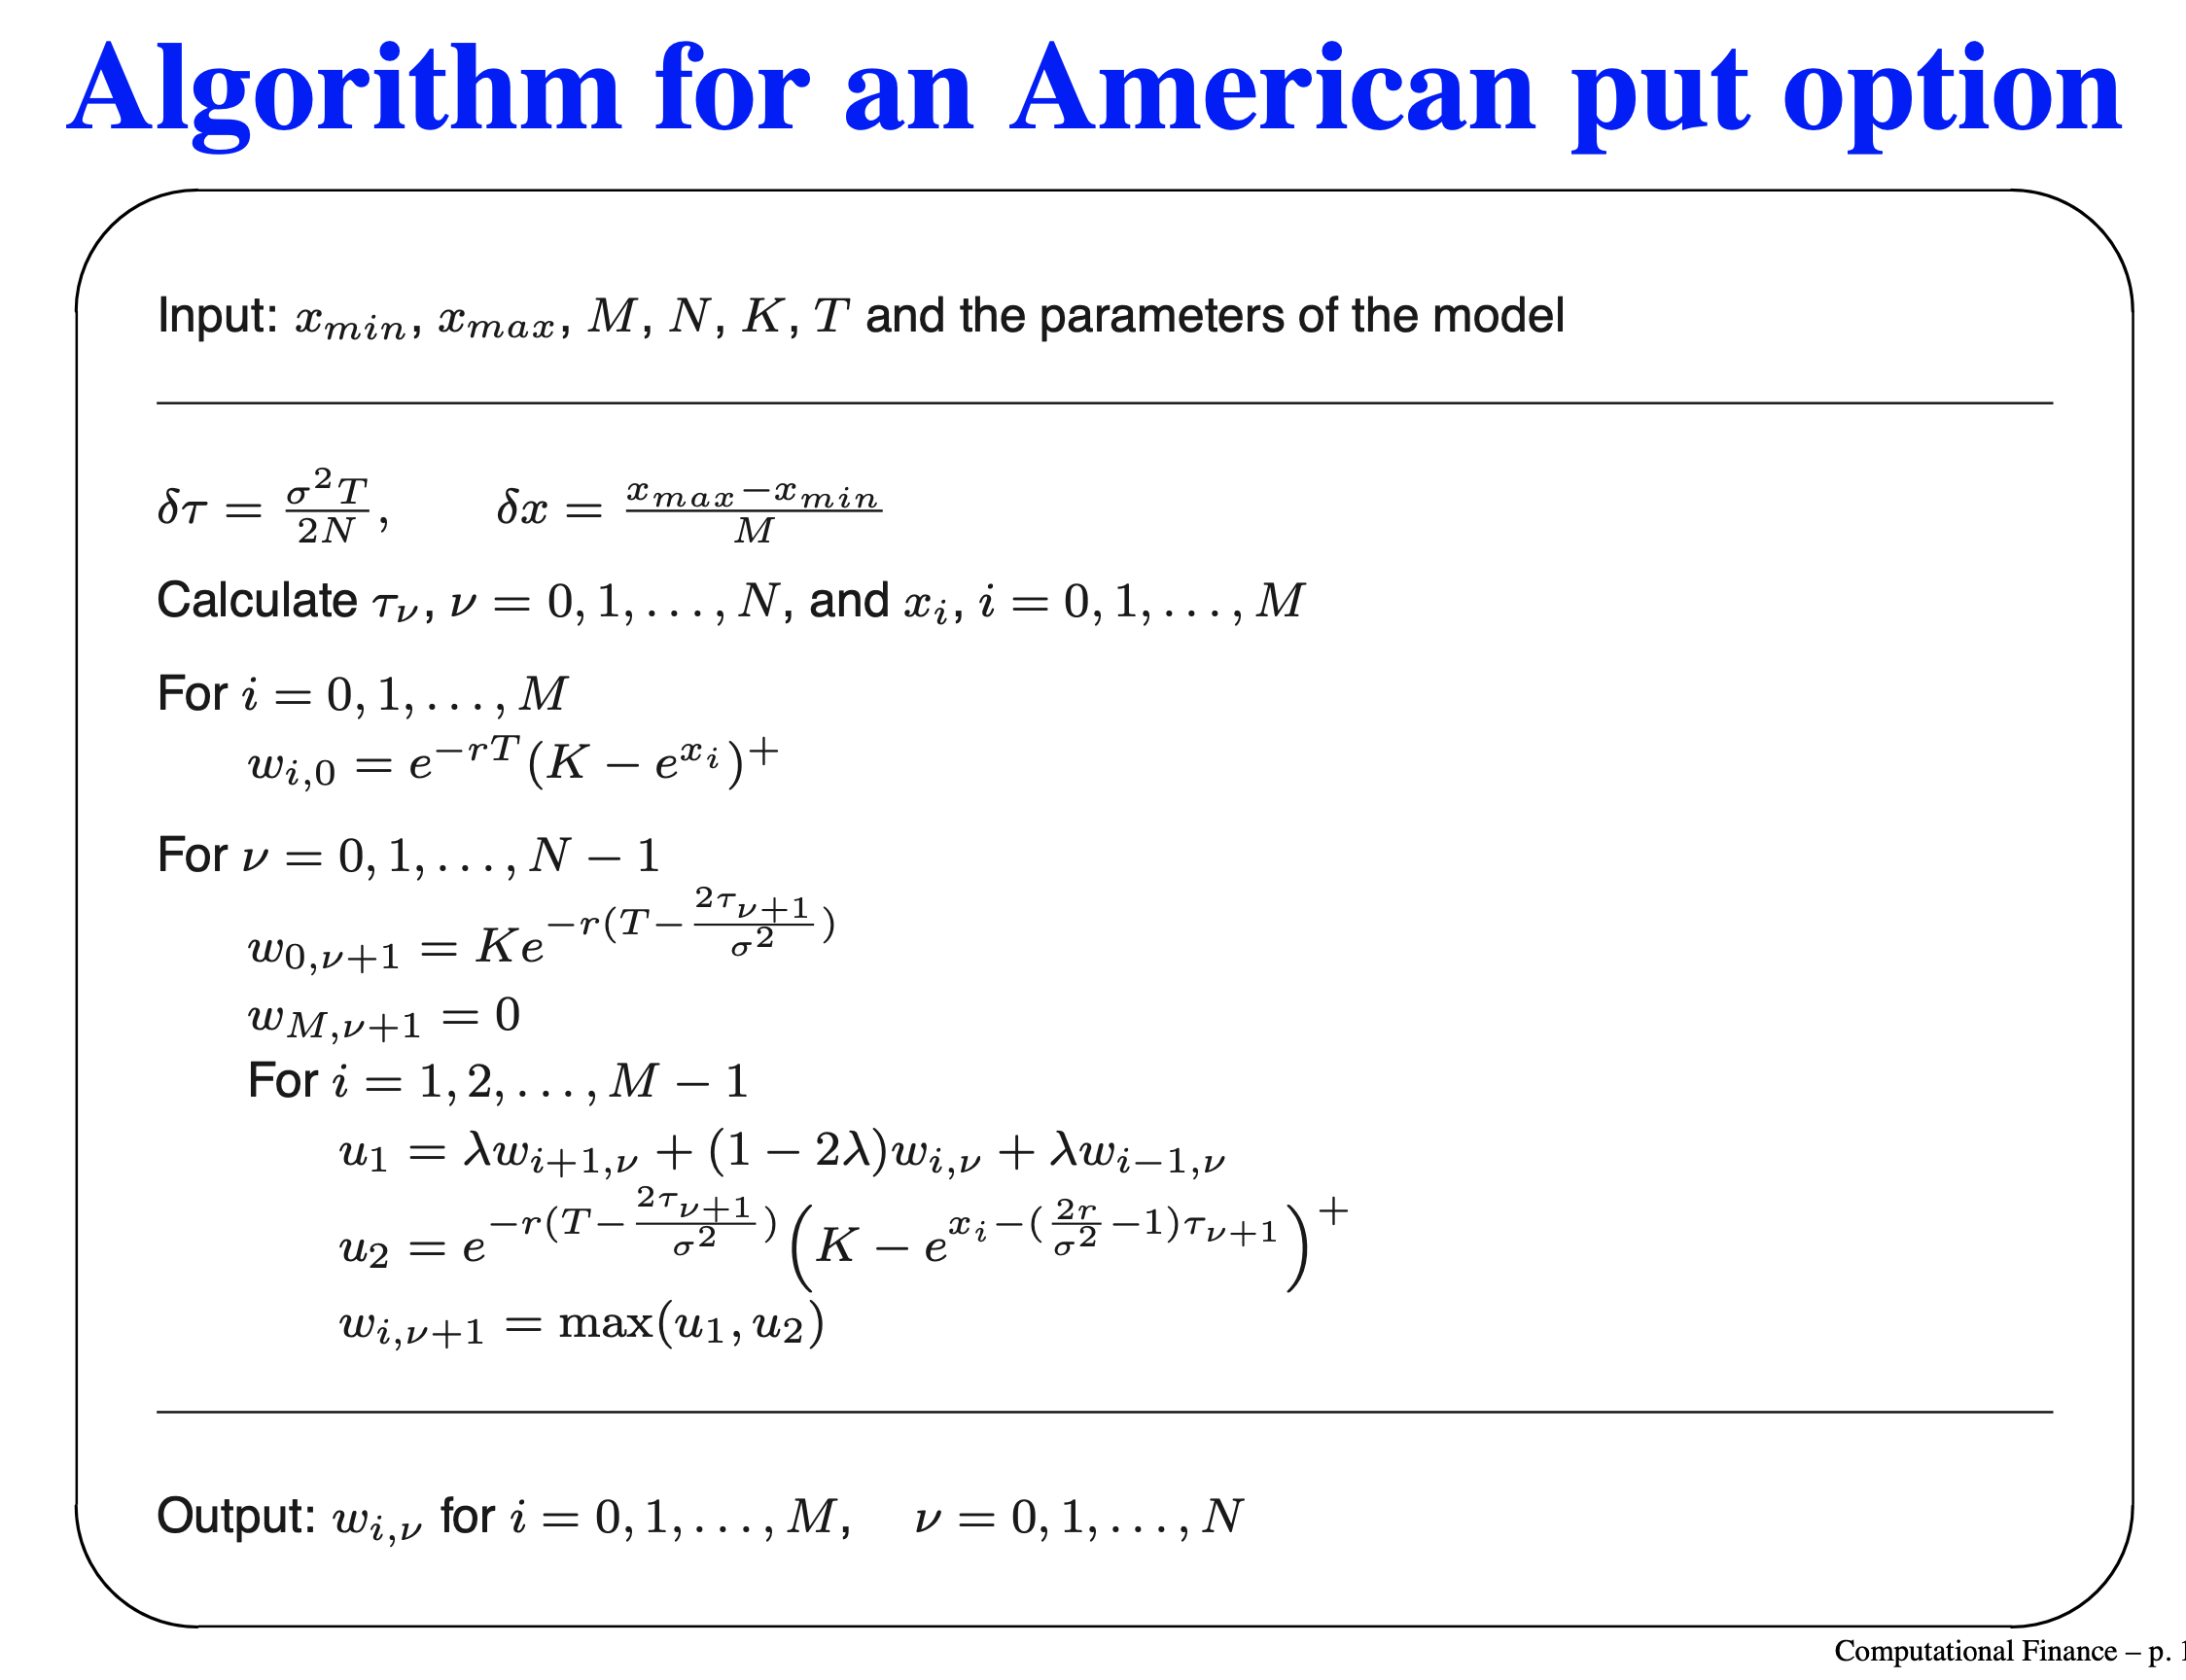
\includegraphics[width = 1.0\linewidth]{palczewski.png}
		\caption[Algorithm - American BS]{Algorithm - American BS}
		\label{fig:Al}
	\end{figure}
	
	\begin{figure}[H]
		\centering
		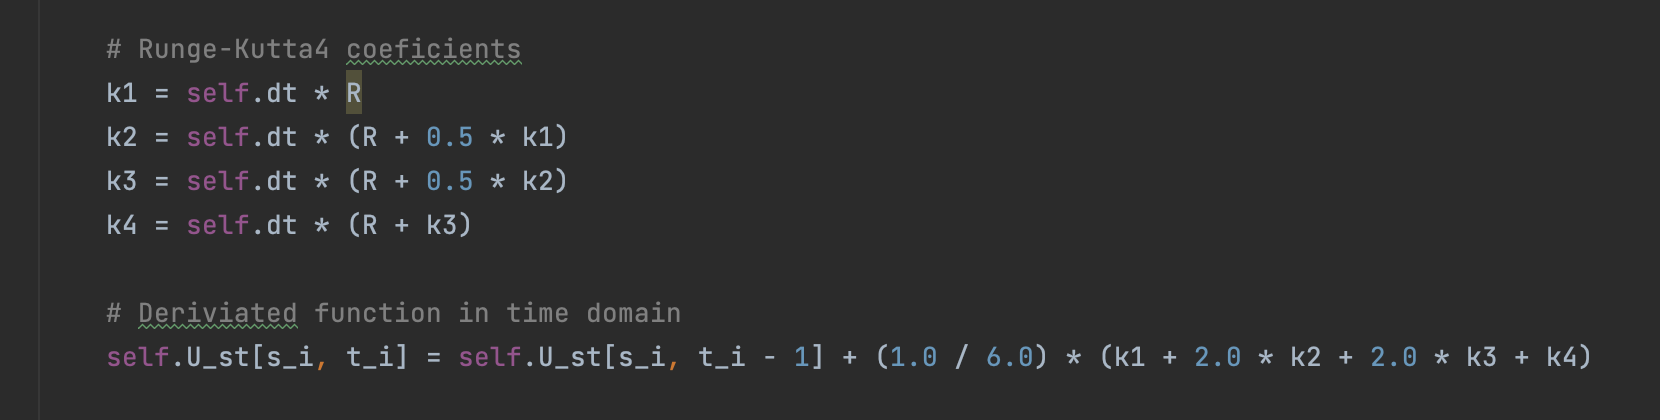
\includegraphics[width = 1.0\linewidth]{european.png}
		\caption[European Option computation]{European Option computation}
		\label{fig:Eu}
	\end{figure}

	\begin{figure}[H]
		\centering
		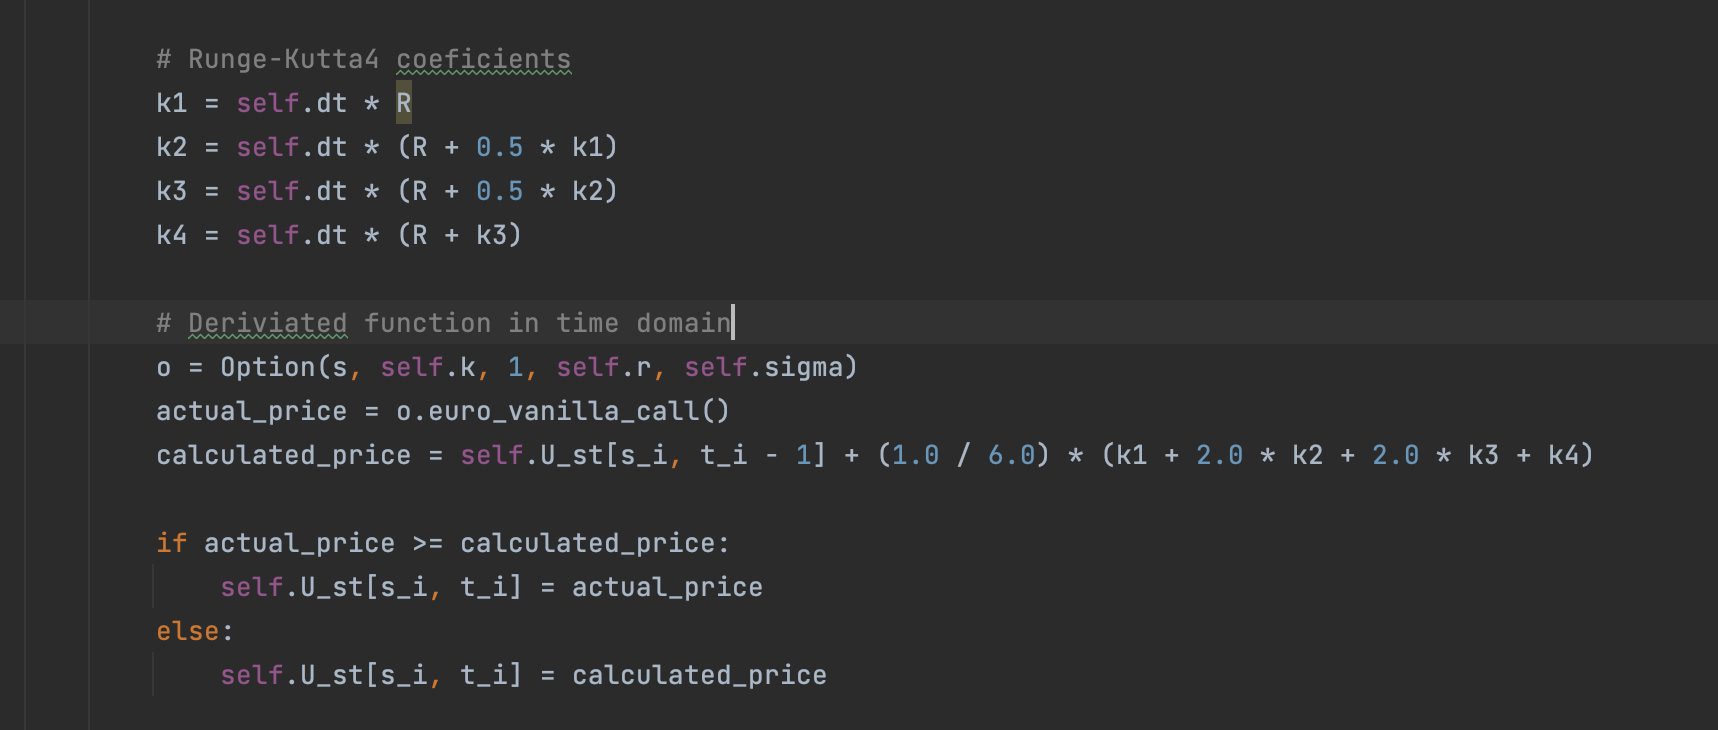
\includegraphics[width = 1.0\linewidth]{american.png}
		\caption[American Option computation]{American Option computation}
		\label{fig:Am}
	\end{figure}

	\begin{table}
	\begin{tabular}{|c|c|}
		\hline
		European & American \\
		\hline
		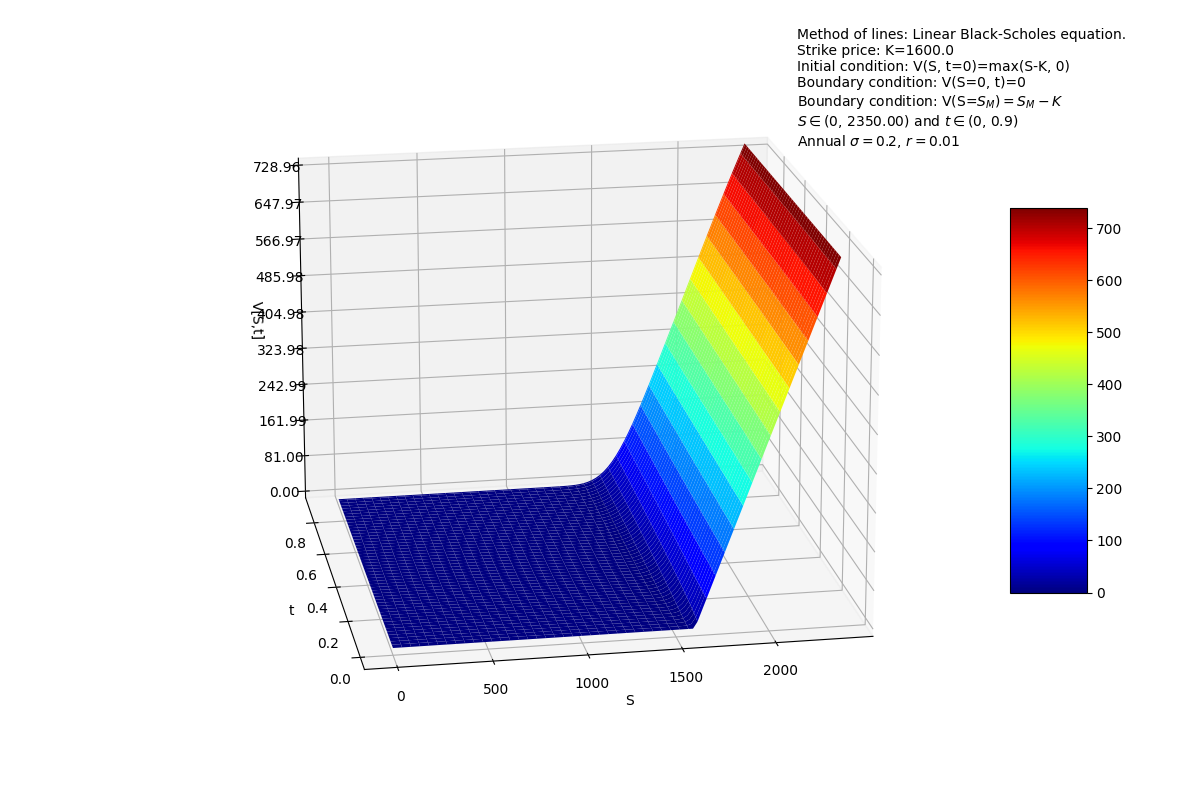
\includegraphics[width=0.5\textwidth, height=40mm]{Black-Scholes_K1600.0_sigma0.2_r0.01_T0.9_linear_european.png}
		& 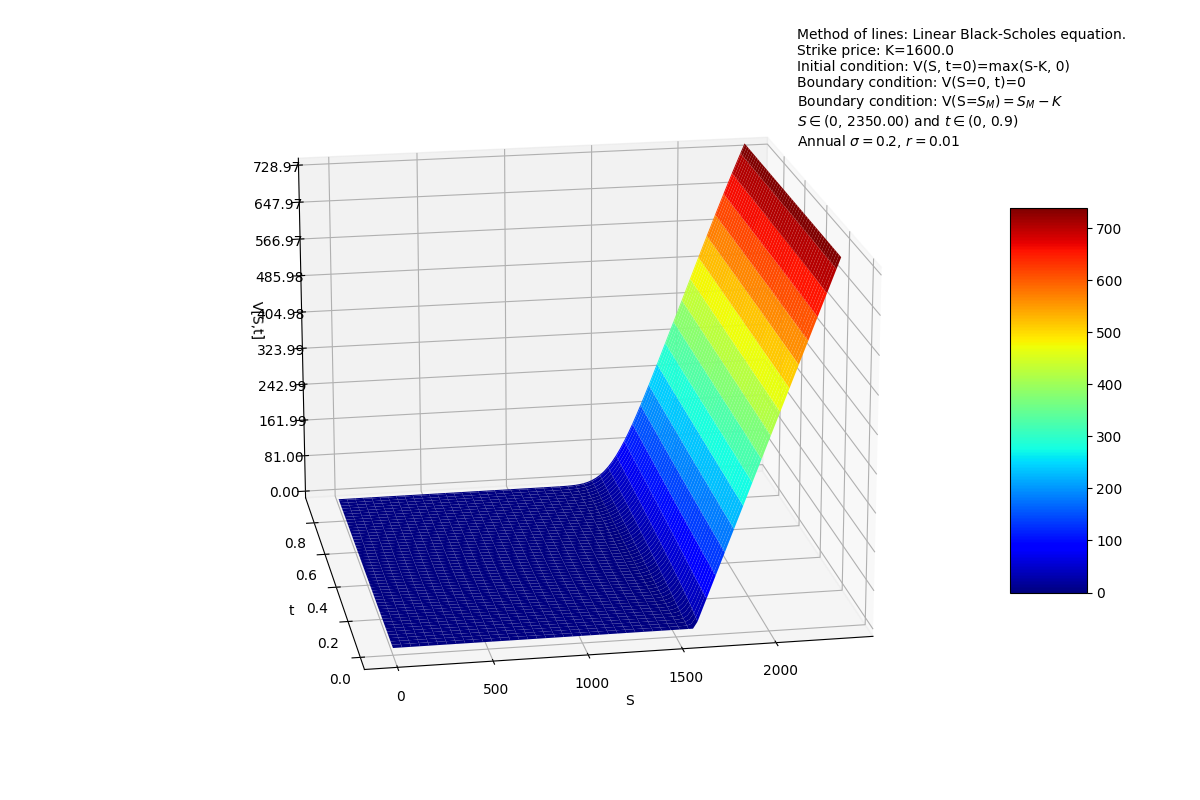
\includegraphics[width=0.5\textwidth, height=40mm]{Black-Scholes_K1600.0_sigma0.2_r0.01_T0.9_linear_american.png} \\
		1.324
		& 1.325 \\

		\hline
		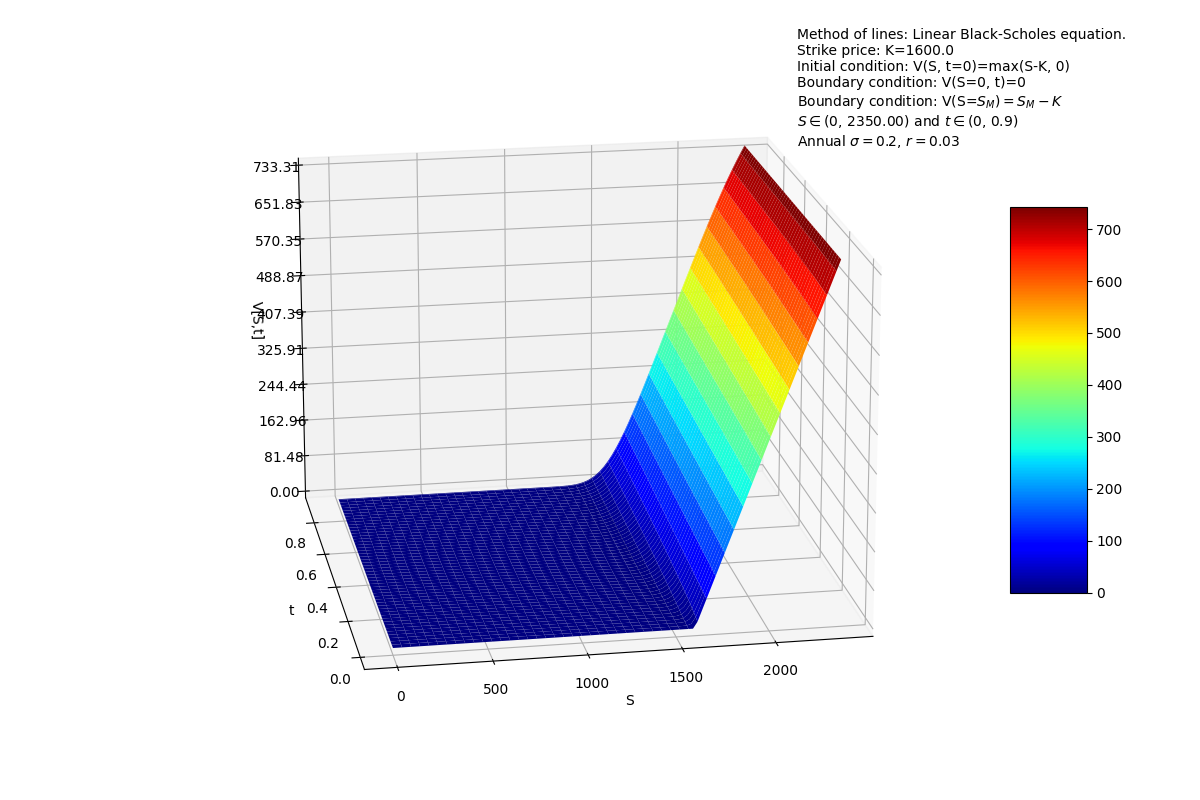
\includegraphics[width=0.5\textwidth, height=40mm]{Black-Scholes_K1600.0_sigma0.2_r0.03_T0.9_linear_european.png}
		& 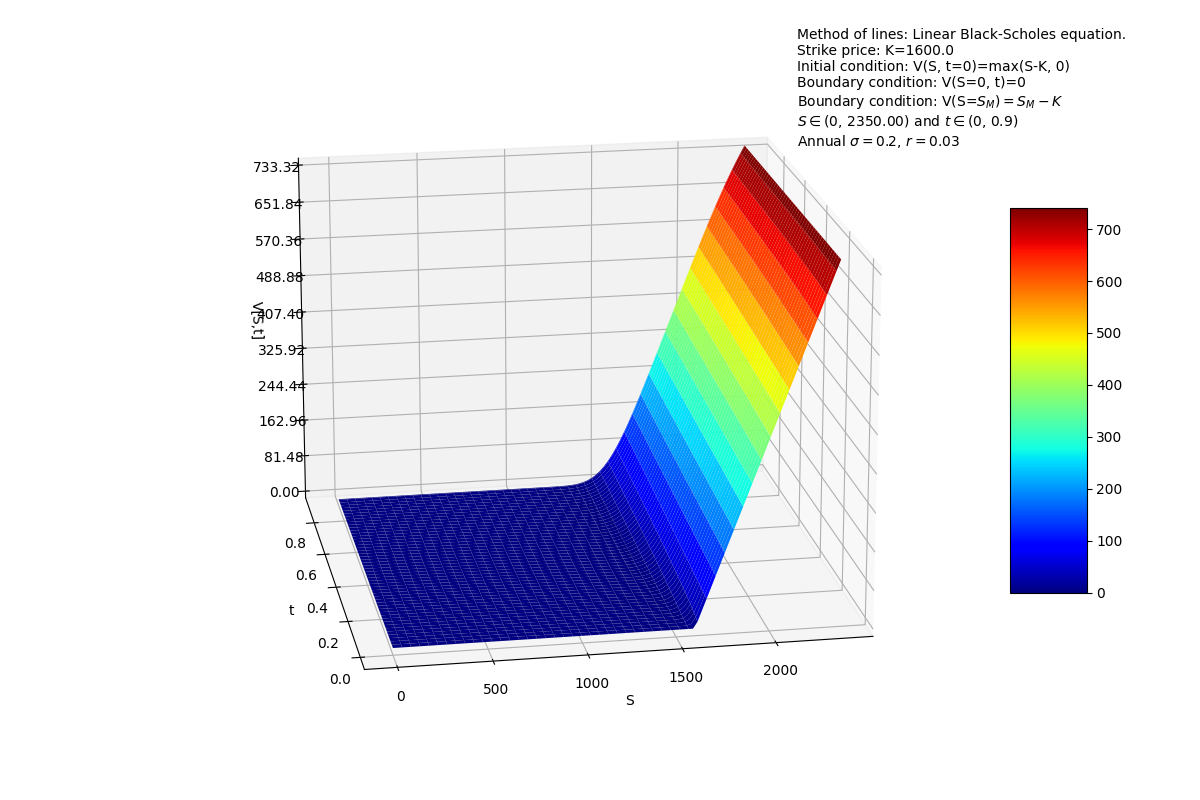
\includegraphics[width=0.5\textwidth, height=40mm]{Black-Scholes_K1600.0_sigma0.2_r0.03_T0.9_linear_american.png} \\
		1.671 &  1.676\\
		\hline
		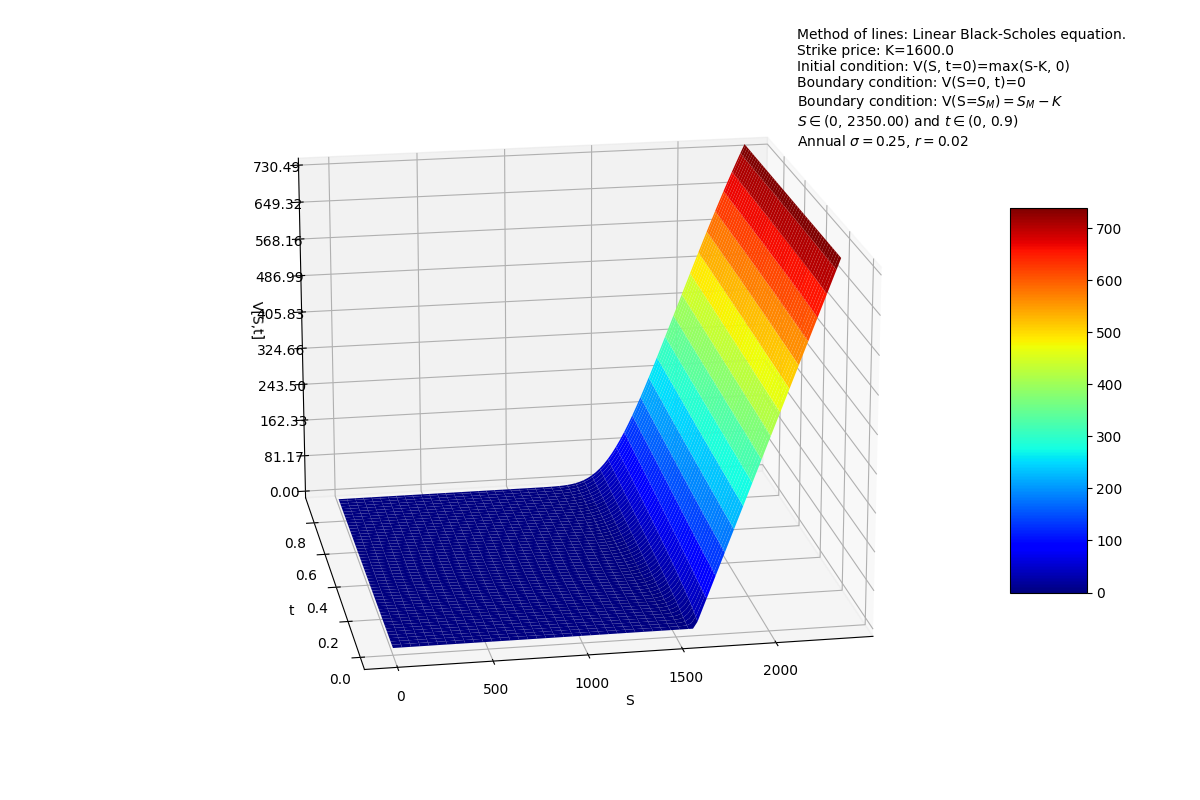
\includegraphics[width=0.5\textwidth, height=40mm]{Black-Scholes_K1600.0_sigma0.25_r0.02_T0.9_linear_european.png}
		& 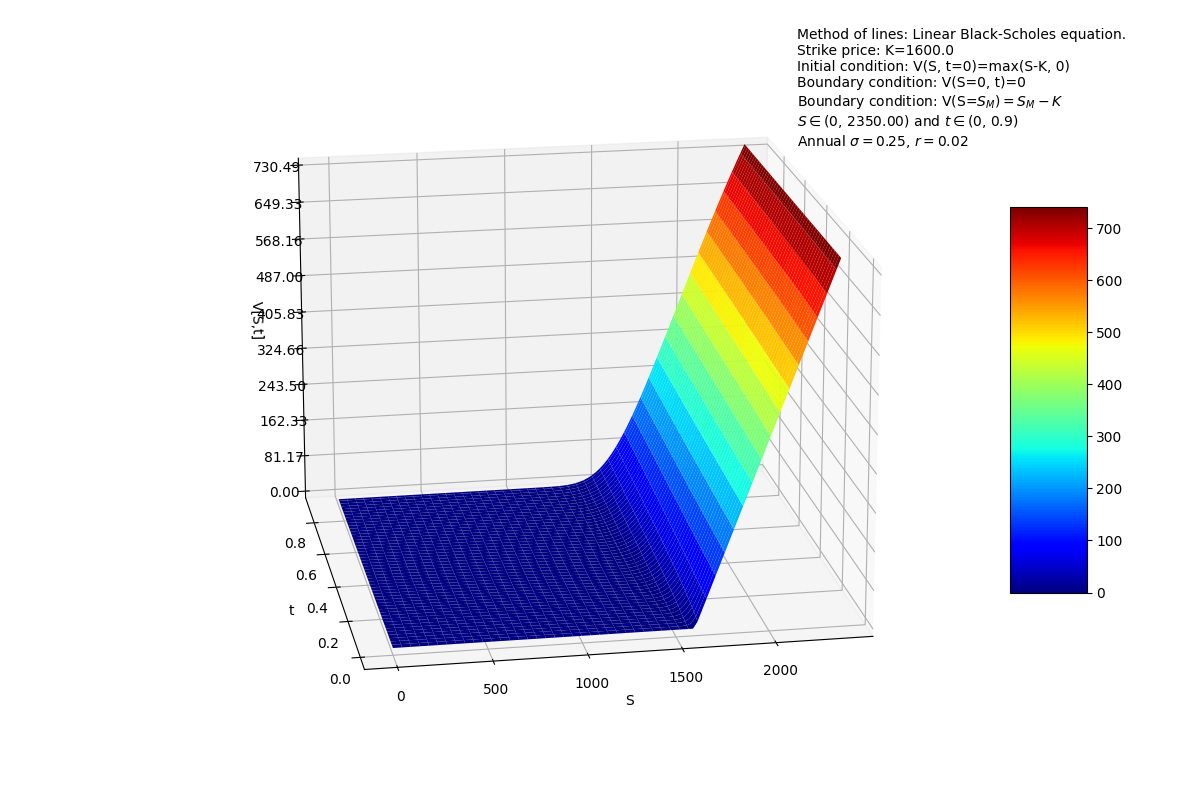
\includegraphics[width=0.5\textwidth, height=40mm]{Black-Scholes_K1600.0_sigma0.25_r0.02_T0.9_linear_american.png} \\
		3.395 & 3.400 \\ 
		\hline
	\end{tabular}
	\caption{Option pricing for European and American style using  linear Black-Scholes model. $S_0=1500$ and $K=1600$}\label{tbl:linear}	
		\end{table}
	
		\begin{table}
		\begin{tabular}{|c|c|}
		\hline
		European & American \\
		\hline
		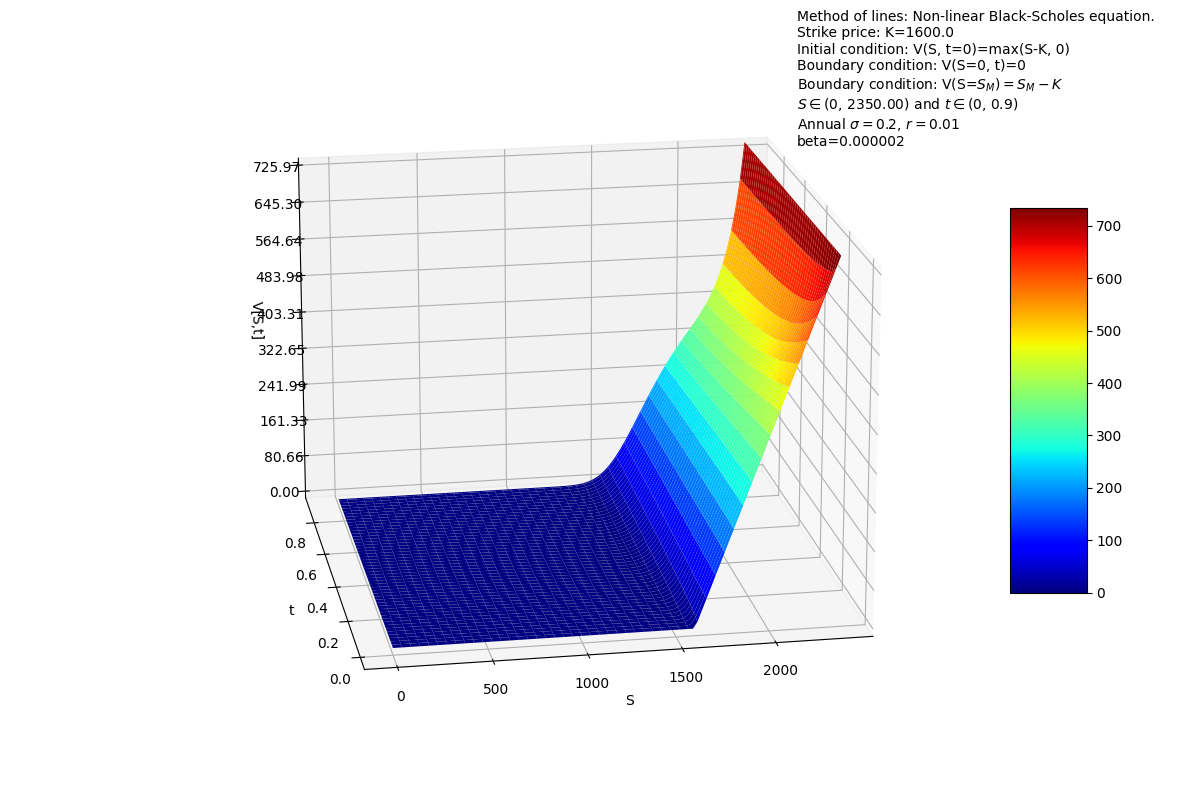
\includegraphics[width=0.5\textwidth, height=40mm]{Black-Scholes_K1600.0_sigma0.2_r0.01_beta2e-06_T0.9_nonlinear_european.png}
		& 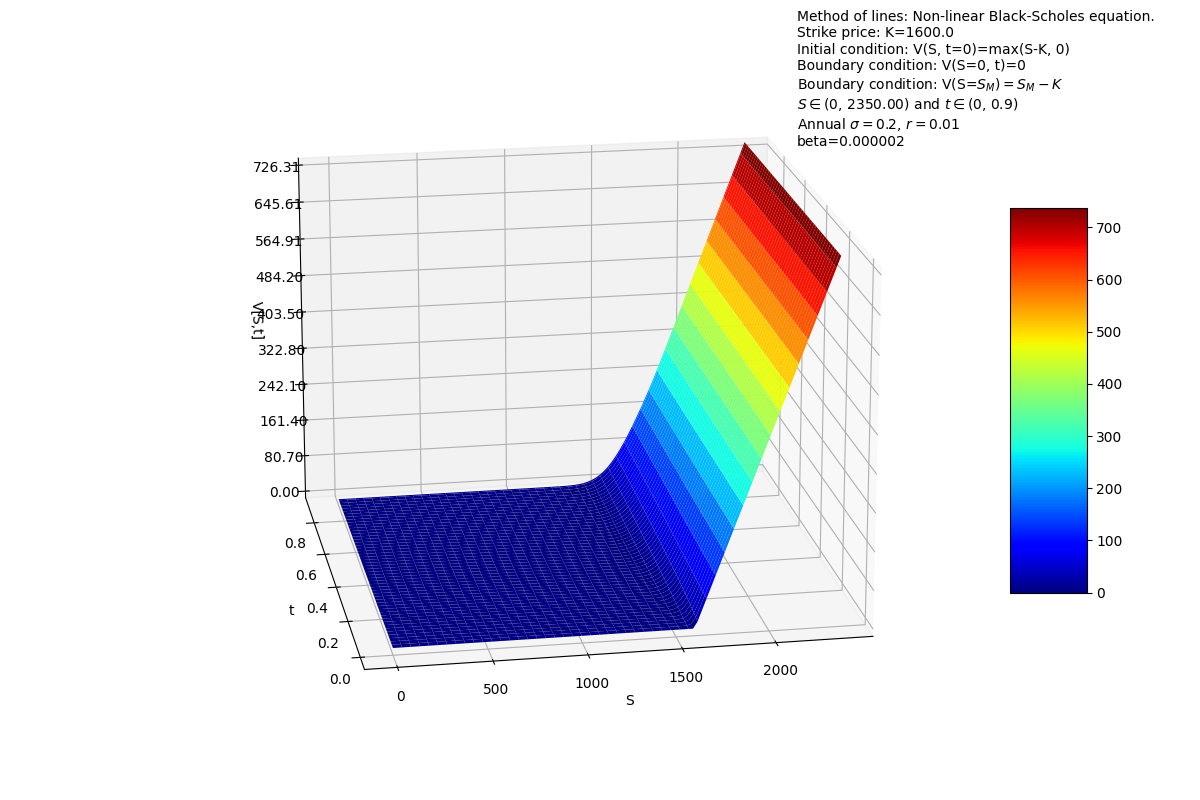
\includegraphics[width=0.5\textwidth, height=40mm]{Black-Scholes_K1600.0_sigma0.2_r0.01_beta2e-06_T0.9_nonlinear_american.png} \\
		1.392
		& 1.392 \\
		
		\hline
		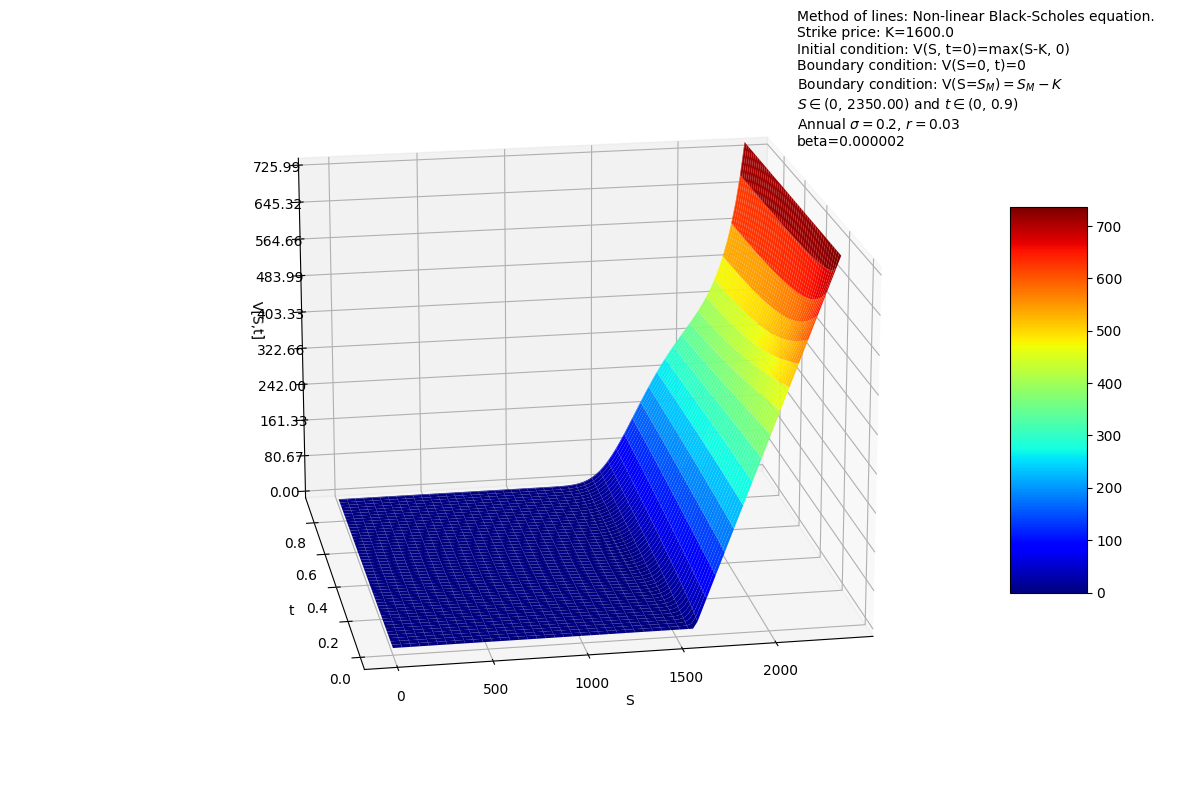
\includegraphics[width=0.5\textwidth, height=40mm]{Black-Scholes_K1600.0_sigma0.2_r0.03_beta2e-06_T0.9_nonlinear_european.png}
		& 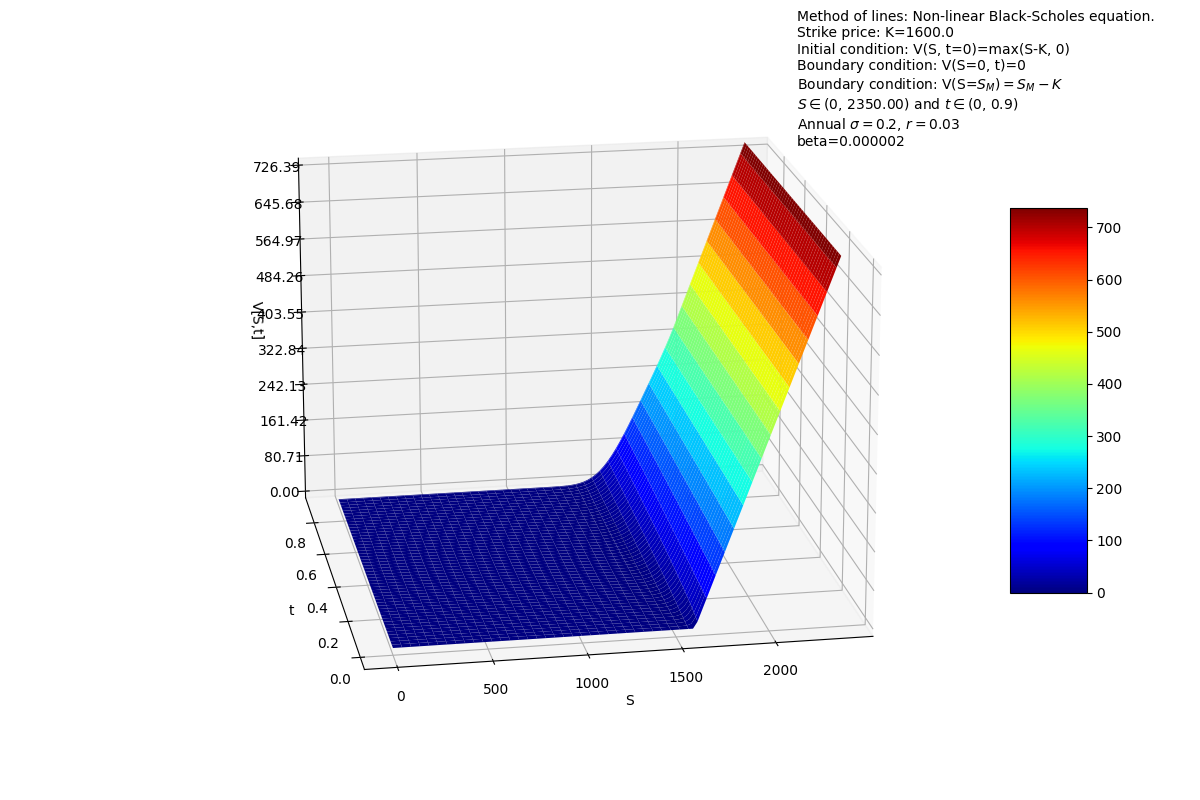
\includegraphics[width=0.5\textwidth, height=40mm]{Black-Scholes_K1600.0_sigma0.2_r0.03_beta2e-06_T0.9_nonlinear_american.png} \\
		1.907 &  1.912\\
		\hline
		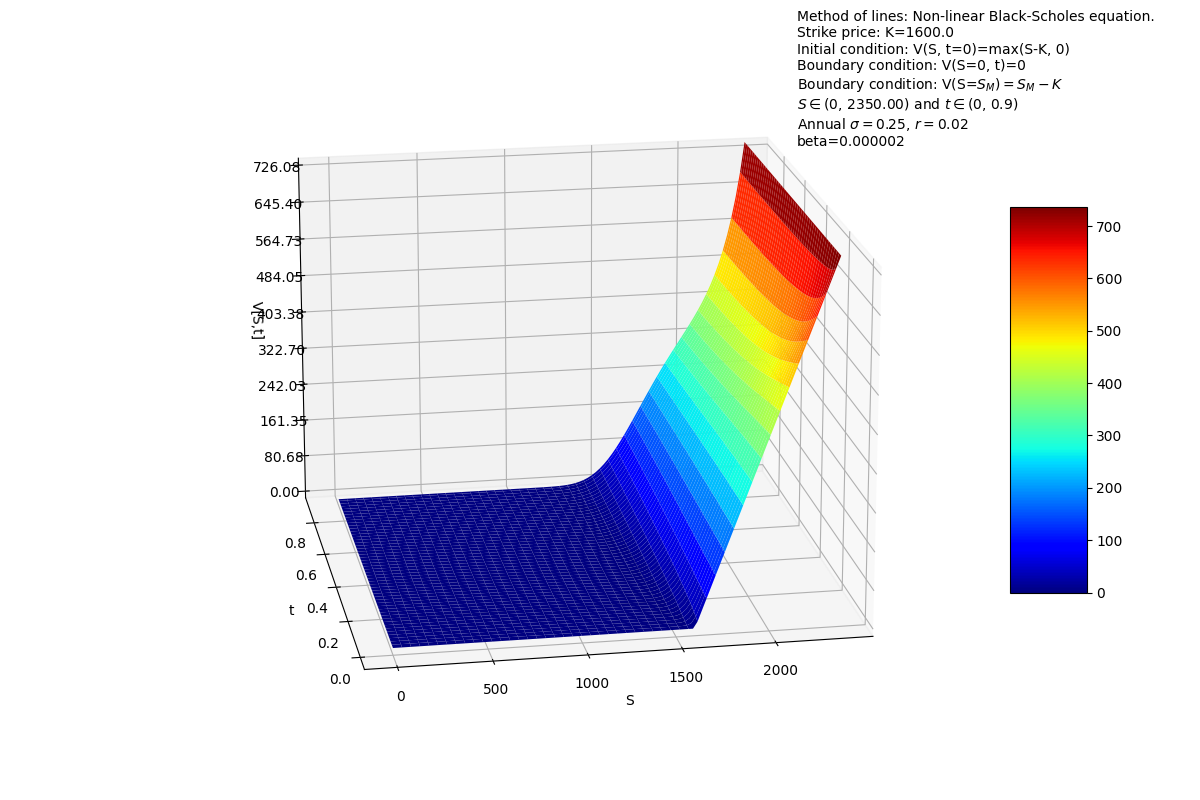
\includegraphics[width=0.5\textwidth, height=40mm]{Black-Scholes_K1600.0_sigma0.25_r0.02_beta2e-06_T0.9_nonlinear_european.png}
		& 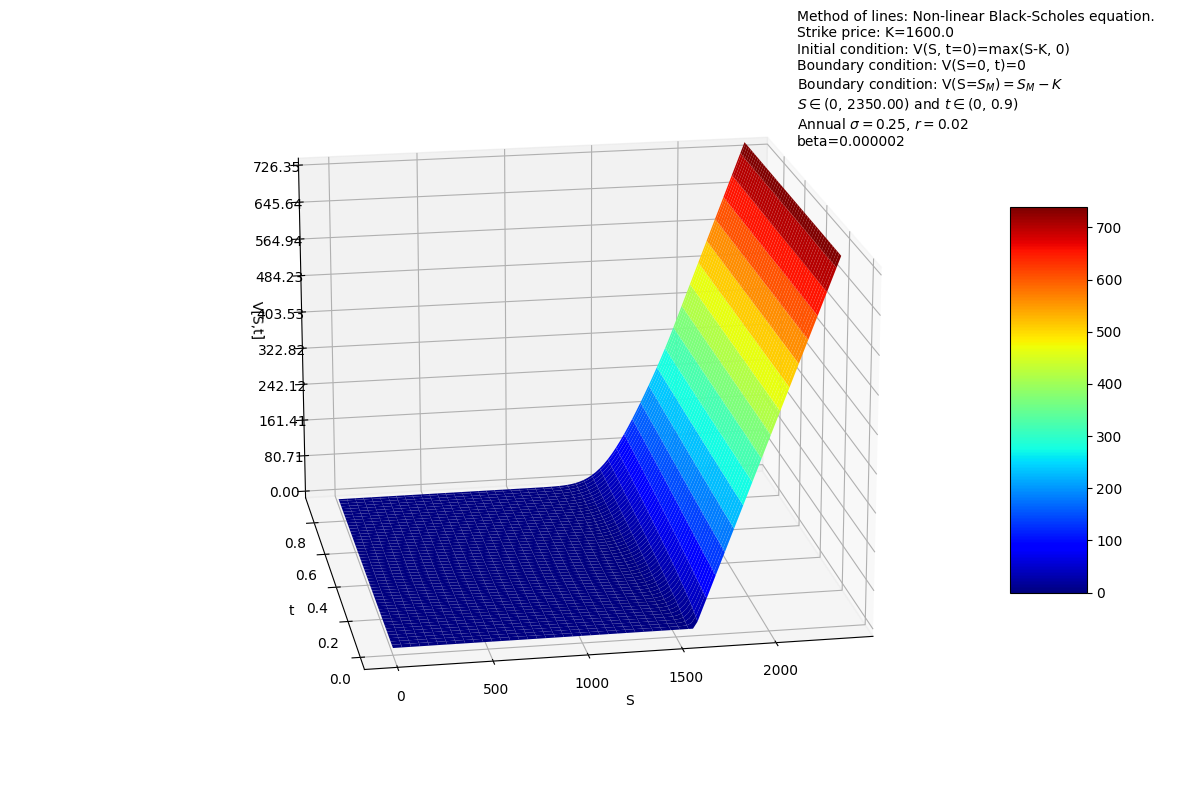
\includegraphics[width=0.5\textwidth, height=40mm]{Black-Scholes_K1600.0_sigma0.25_r0.02_beta2e-06_T0.9_nonlinear_american.png} \\
		3.570 & 3.575 \\ 
		\hline
	\end{tabular}
	\caption{Option pricing for European and American style using  non-linear Black-Scholes model. $S_0=1500$ and $K=1600$}\label{tbl:nonlinear}	
\end{table}

\end{document}